\begin{picture}(0,0)%
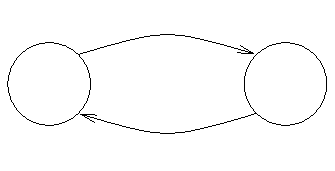
\includegraphics{figures/updown-automaton}%
\end{picture}%
\setlength{\unitlength}{4144sp}%
%
\begingroup\makeatletter\ifx\SetFigFont\undefined%
\gdef\SetFigFont#1#2{%
  \fontsize{#1}{#2pt}%
  \selectfont}%
\fi\endgroup%
\begin{picture}(2550,1296)(976,-1174)
\put(3151,-556){\makebox(0,0)[b]{\smash{{\SetFigFont{12}{14.4}{\color[rgb]{0,0,0}Down}%
}}}}
\put(3511,-556){\makebox(0,0)[lb]{\smash{{\SetFigFont{12}{14.4}{\color[rgb]{0,0,0}\lstinline{x = last x - 1}}%
}}}}
\put(1351,-556){\makebox(0,0)[b]{\smash{{\SetFigFont{12}{14.4}{\color[rgb]{0,0,0}Up}%
}}}}
\put(991,-556){\makebox(0,0)[rb]{\smash{{\SetFigFont{12}{14.4}{\color[rgb]{0,0,0}\lstinline{x = last x + 1}}%
}}}}
\put(2251,-61){\makebox(0,0)[b]{\smash{{\SetFigFont{12}{14.4}{\color[rgb]{0,0,0}$\mathtt{x} \geq 10$}%
}}}}
\put(2251,-1096){\makebox(0,0)[b]{\smash{{\SetFigFont{12}{14.4}{\color[rgb]{0,0,0}$\mathtt{x} \leq 0$}%
}}}}
\end{picture}%
